\documentclass[a4paper,12pt]{article}
\usepackage[margin=1in]{geometry}
\usepackage{enumerate}
\usepackage{tikz}
\usepackage{subcaption}
\usepackage{float}
\usepackage[bottom]{footmisc}
\usepackage{hyperref}
\usepackage{amsfonts}
\usepackage{amsmath}
\usepackage{graphicx}
\usepackage[backend=biber,style=mla,sorting=ynt]{biblatex}
\usepackage{listings}
\usepackage{xcolor}
\usepackage{setspace}

\lstset { %
    language=C++,
    backgroundcolor=\color{black!5}, % set backgroundcolor
    basicstyle=\footnotesize,% basic font setting
}
\addbibresource{citations.bib}
\newtheorem{lemma}{Lemma}
\newtheorem{sublemma}{Lemma}[lemma]
\newtheorem{theorem}{Theorem}

\usetikzlibrary{graphs} 
\usetikzlibrary{graphdrawing}
\usetikzlibrary{graphs.standard}
\usetikzlibrary{positioning}
\usegdlibrary{layered,circular,force}
\title{Hamiltonian Cycles in Square Lattice Graphs}
\begin{document}
\date{\vspace{-5ex}}
\maketitle
\tableofcontents
\doublespacing

\section{Abstract}
This paper identifies a visual property of boundaries of right-angled walls, found in the video game Pac-Man, where corners are rounded and walls are straight and oriented towards with the normal of the path which they face, and connected to neighbouring walls. The walls form a closed boundary. The 2-dimensional gridded nature of wall placement allows them to be represented using a square lattice graph. With the aim of finding the direction towards which they are clamped, so as to recreate the visual properties of the walls in Pac-Man, we devise a polynomial-complexity algorithm for finding a hamiltonian cycle in square-lattice subgraphs. The algorithm will be tested in a program written by the author in the C and Objective C programming language, deriving the resultant image demonstrating the algorithm's outcome. 

\section{Problem Introduction}
Pacman is a video game which utilizes individual textures of 8x8 pixels to render its core components as can be seen in Figure~\ref{PacmanLevelGrid}, each respectively represented by one square in the dotted grid.

\begin{figure}[H]
\centering
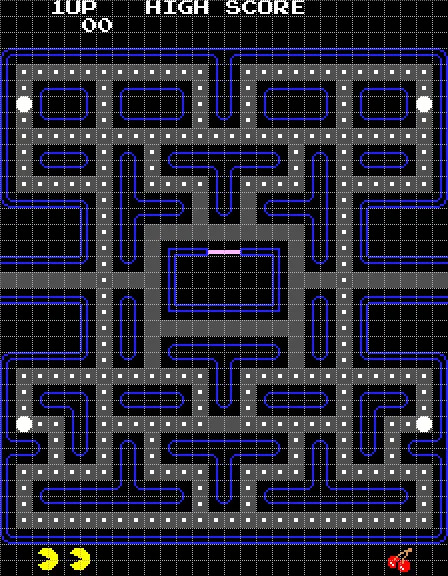
\includegraphics[width=0.4\linewidth]{Image-1.jpg}
\caption {Pacman level divided into squares of 8x8 pixels.\autocite{pittman_pac-man_2009}}\label{PacmanLevelGrid}
\end{figure}

Since the pixel length of a wall is 1 pixel, the wall textures all contain an asymmetry over the central vertical line as seen in Figure~\ref{StraightWallTexture} and~\ref{CornerTexture}. The asymmetry is the basis of the visual appearance of levels which are formed by an oriented placing of these textures. 

\begin{figure}[H]
\centering
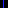
\includegraphics[width=0.4\linewidth]{Image-2.png}
\caption {A single wall texture. As can be seen this wall is clamped to the right, and would connect a tile above it and below it.\autocite{myself}}\label{StraightWallTexture}
\end{figure}

\begin{figure}[H]
\centering

\includegraphics[width=0.4\linewidth]{Image-3.png}
\caption {Square texture of a corner.\autocite{myself}}\label{CornerTexture}
\end{figure}

Because of this asymmetry, it must be decided in what direction walls are clamped, that is in what direction the asymetry should act to ensure visual consistency. When all walls are clamped in the same direction we receive unsatisfactory results as seen on the left part of Figure~\ref{WallTextureAsymmetry}. 

\begin{figure}[H]
\centering
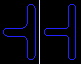
\includegraphics[width=0.4\linewidth]{Image-4.png}
\caption {Left - Incorrect orientation of tiles. Right - Correct orientation with walls clamped to appropriate direction. Walls on the left are clamped inward, to the right and walls on the right are clamped inwards to the left. The problem consists of determining which direction points "inwards" for each tile.\autocite{myself}}\label{WallTextureAsymmetry}
\end{figure}

\begin{figure}[H]
\centering
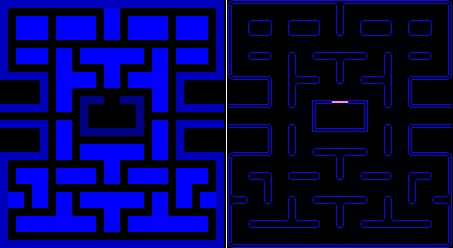
\includegraphics[width=0.8\linewidth]{Image-5.png}
\caption {The algorithm devised through this paper will interpret from the image on the left to the one on the right, reconstructing the visual properties using a simplified outline, only describing the position of the walls.\autocite{myself}}\label{LevelWallConversion}
\end{figure}

This problem will be represented using concepts of graph theory.

\section{Definitions}

\begin{enumerate}[I.]
\item We define a \textit{\textbf{graph}} as a set $G=(V,E)$.\footnote{\autocite{p._bogart_introductory_2000} p. 201.} $V$ is a set of vertices. $E$ is a set of edges. Vertices can be thought of as standalone points. Edges are connections between vertices, where an edge $e\in E, $ for $ V_{x},V_{y}\in V, e=\lbrace V_{x},V_{y} \rbrace $, connects vertices $V_{x}$ and $V_{y}$.  A graph can be represented by a drawing. For the example graph $G=(E,V)$, where $E=\lbrace a,b,c,d \rbrace $ and $ V=\{\{a,b\},\{b,c\},\{c,d\},\{a,d\}\}$ we can draw the following diagram.

\begin{figure}[H]
	\centering
	\tikz [every node/.style={draw,circle}]
		\graph [simple necklace layout, node distance=2cm] {
			a--b--c--d--a
	};
	\caption{A graph of four vertices that are joined together in a loop.\autocite{myself}}\label{NecklaceGraph}
\end{figure}

Here are several other examples of graphs (these are not essential to the paper, but can give a broader idea of what a graph can be):

\begin{figure}[H]
	\centering
	\tikz [every node/.style={draw,circle}] \graph {a--b--c--d};
	\caption{A "spine". \autocite{myself}}\label{SpineGraph}
\end{figure}

\begin{figure}[H]
	\centering
	\tikz [every node/.style={draw,circle}] \graph { subgraph K_n [n=6, clockwise] };
	\caption { A complete graph. \autocite{myself}}\label{CompleteGraph}
\end{figure}

\begin{figure}[H]
	\centering
	\tikz [every node/.style={draw,circle}] \graph { a -> {b, c} -> d };
	\caption {A directed graph. Each edge is assigned a direction indicated by the arrows.\autocite{myself}}\label{DirectedGraph}
\end{figure}

\item We define the \textit{\textbf{degree}} of a vertex $v\in V, d(v)$ as the number of edges $e\in E$ that connect to $v$, for graph $G=(V,E)$.\footnote{\autocite{p._bogart_introductory_2000} p. 205.} In Figure~\ref{CompleteGraph}, all vertices have the same degree as they are all connected to 5 vertices, respectively, where as in Figure~\ref{SpineGraph}, vertex $b$ has a degree $d(b)=2$, whilst $a$ has a degree $d(a)=1$. 

\item A \textit{\textbf{walk}} for a graph $G=(V,E)$ is an alternating sequence of vertices in $V$ and edges in $E$.\footnote{\autocite{p._bogart_introductory_2000} p. 204.} It has the form ${v_1}{e_1}{v_2}{e_2}{v_3}{e_3}...{e_{n-1}}{v_n}$, where $e_k\in E,v_l\in V, 1\leq k\leq n-1, 1\leq l\leq n$, and $e_k$ is an edge between $v_k$ and $v_{k+1}$. A walk in which only the first and last vertices are equal, is called a \textit{\textbf{cycle}}.\footnote{\autocite{p._bogart_introductory_2000} p. 204} The following diagrams are examples of walks:

\begin{figure}[H]
	\centering
	\tikz [every node/.style={draw,circle}] \graph [simple, grow right=2cm] {
		 subgraph K_n [n=6, clockwise];
 		 {[edges={red,thick}] 1 ->  2 -> 5 -> 3 -> 4 -> 6}
	};
	\caption {A path with vertices 1,2,5,3,4,6, and the respective edges to join them.\autocite{myself}}\label{FiniteWalk}
\end{figure}

\begin{figure}[H]
	\centering
	\tikz [every node/.style={draw,circle}] \graph [grid placement] { 
		subgraph Grid_n [n=9];

		{[edges={red,thick}] 1 -> 2 -> 3 -> 6 -> 5 -> 8 -> 7 -> 4 -> 1}
	};
	\caption {A path with vertices 1,2,3,6,5,8,7,4,1. The walk comes back to the first vertex through a string of unique vertices and is thus a cycle.\autocite{myself}}\label{CycleWalk}
\end{figure}

\item A \textit{\textbf{Hamiltonian cycle}} for a graph $G=(V,E)$ is a cycle containing every vertex $v\in V$.\footnote{\autocite{p._bogart_introductory_2000} p. 210} Since it is a cycle, it comes back to the first vertex of the walk, but, by definition, does not walk onto the any other vertex on more than one occasion. The following is an example of a hamiltonian cycle:

\begin{figure}[H]
	\centering
	\tikz [every node/.style={draw,circle}] \graph [grid placement, grow down=1.5cm, branch right=1.5cm, ] { 
		subgraph Grid_n [n=36];
		{[edges={red,line width=2pt}] 1 -> 2 -> 3 -> 9 -> 15 -> 16 -> 10 -> 4 -> 5 -> 6 -> 12 -> 11 -> 17 -> 18 -> 24 -> 23 -> 29 -> 30 -> 36 -> 35 -> 34 -> 28 -> 22 -> 21 -> 27 -> 33 -> 32 -> 31 -> 25 -> 26 -> 20 -> 19 -> 13 -> 14 -> 8 -> 7 -> 1}
	};
	\caption {A Hamiltonian cycle. Although it does not include every edge, it includes each vertex exactly once, before arriving at the starting vertex (Note that the starting vertex is abritrary as the path is a loop; any vertex can be considered the starting vertex).\autocite{myself}}\label{HamiltonianCycle}
\end{figure}

\item A \textit{\textbf{square lattice}} graph $G=(V,E)$ is a graph in which each vertex can be distinctly mapped onto an integer tuple $(x,y)$, where $x,y\in \mathbb{Z}$, and where the edges of a vertex $v\in V$ only connect to the respective vertices of a distance of 1 in each cardinal direction. Essentially, a square lattice graph is a graph created out of some points on a coordinate grid, that for a coordinate $(x,y)$ are only ever connected by edges to coordinates with coordinate points $(x+1,y), (x-1,y), (x,y+1)$, or $(x,y-1)$. Figures~\ref{NecklaceGraph},~\ref{SpineGraph},~\ref{CycleWalk}, and~\ref{HamiltonianCycle} are all examples of square lattice graphs.

\end{enumerate}

\section{Observations}
We will first focus on the smaller components, that is individual collections of walls, that fill most of the interior of the level blueprint of Figure ~\ref{LevelWallConversion}.
\begin{enumerate}[I.]
\item Firstly, we observe that walls are oriented away from the path they face as can be seen in Figure~\ref{PathNormal}. The walls connect to neighbours, and non-corner walls face into the normal of the direction of the path. Because of the walls' asymmetry there are two different ways to face the path, one ''clamped'' towards and one away. Consistently clamping in the same direction establishes the visual conditions of the walls. Thus the problem reduces to finding normal of the wall square's adjacent path, and consistently clamping away in relation to it.
\begin{figure}[H]
	\centering
	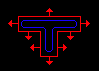
\includegraphics[width=0.4\linewidth]{Image-6.png}
	\caption {Arrows show the normal to the path that surrounds the boundary formed by the walls.\autocite{myself}} \label{PathNormal}
\end{figure}

\item To find the normal to the direction of the path around the walls, we must first know the direction of the path adjacent to each wall square. Since the walls, forming the boundary, define the path that surrounds, as they serve as an outline of it, we must find the closed path which the walls themselves form.\label{ClosedPathObservation} Instead of using the path adjacent to the walls as a rule of determining the tiles' orientation, we will use the tiles themselves in relation to each other, to trace their boundary thus finding the normal of that outline and solving the problem.

\item Since the walls each represent a single square in a rectangular 2D grid of integer coordinates, we can map them onto a square lattice graph as can be seen in Subfigure~\ref{BoundaryLattice}.\label{SquareLatticeObservation}

\begin{figure}[H]
	\begin{subfigure}[b]{0.5\textwidth}
		\centering
		
\includegraphics[width=0.7\linewidth]{Image-7.png}
		\caption {Pixel representation of a boundary formed by walls.\autocite{myself}}\label{PixelBoundary}
	\end{subfigure}
	\begin{subfigure}[b]{0.5\textwidth}
		\centering
		\tikz[every node/.style={draw,circle}] \graph [no placement] {
			a [x=0,y=3] -- b [x=1,y=3] -- c[x=2,y=3] -- d[x=3,y=3] -- e[x=4,y=3] -- f[x=5,y=3] -- g[x=5,y=2] -- h[x=4,y=2] -- i[x=3,y=2] -- j[x=3,y=1] -- k[x=3,y=0] -- l[x=2,y=0] -- m[x=2,y=1] -- n[x=2,y=2] -- o[x=1,y=2] -- p[x=0,y=2] -- a;
			b -- o;
			c -- n;
			d -- i;
			e -- h;
			n -- i;
			m -- j;
		};
		\caption {Corresponding lattice graph of the wall configuration in~\ref{PixelBoundary}\autocite{myself}}\label{BoundaryLattice}
	\end{subfigure}
	\caption {Two representations of graph boundaries.}
\end{figure}

\item We can find a Hamiltonian cycle of the square lattice of the walls of a Pacman level to find the path defining its boundary to solve the problem, accounting for observations~\ref{ClosedPathObservation} and~\ref{SquareLatticeObservation}.

\begin{figure}[H]
	\centering
	\tikz[every node/.style={draw,circle}] \graph [no placement] {
		a [x=0,y=3] -> b [x=1,y=3] -> c[x=2,y=3] -> d[x=3,y=3] -> e[x=4,y=3] -> f[x=5,y=3] -> g[x=5,y=2] -> h[x=4,y=2] -> i[x=3,y=2] -> j[x=3,y=1] -> k[x=3,y=0] -> l[x=2,y=0] -> m[x=2,y=1] -> n[x=2,y=2] -> o[x=1,y=2] -> p[x=0,y=2] -> a;
		b -- o;
		c -- n;
		d -- i;
		e -- h;
		n -- i;
		m -- j;
		{[edges={red,line width=2pt}] a->b->c->d->e->f->g->h->i->j->k->l->m->n->o->p->a}
	};
	\caption {Desired Hamiltonian cycle for lattice graph in Figure~\ref{BoundaryLattice}}\label{HamiltonianBoundaryLattice}
\end{figure}

\end{enumerate}

\section{Properties of Square Lattice Graphs}
\begin{theorem}
Every vertex $v\in V$ of a square lattice graph $G=(V,E)$ representing a closed boundary, must have a degree $d(v)\geq 2$.\label{DegreeLemma}
\end{theorem}
\subsubsection*{Proof of Theorem~\ref{DegreeLemma}}
If a vertex $v\in V$ has degree $d(v)=0$, and the number of vertices $\in V$, $n>1$, then that vertex cannot connect to any other vertices in the square lattice graph, and can thus not form part of the closed boundary. If a vertex $v_0\in V$ has degree $d(v_0)=1$, then any path $p$ where $v\in p$, will not be a Hamiltonian cycle, as the edge $e\in E$ where $v_0\in e$, can only be crossed once, as the adjacent vertex $v_1\in e$, can only be crossed once on path $p$.
\begin{theorem}
In a square lattice graph of a closed boundary wall configuration, in relation to the vertices' grid coordinates, out of the northernmost vertices, the westmost vertex will always be a corner connecting two vertices to its east and its south, respectively.\label{NorthwestCornerLemma}
\end{theorem}
\subsubsection*{Proof of Theorem~\ref{NorthwestCornerLemma}}
In such a lattice graph, we pick the westmost vertex amongst the northernmost vertices. If there is a vertex connected to it, to its north, then our chosen vertex was not the northernmost vertex which is a contradiction. If there is a vertex connected to its west, then it is not the westmost vertex and is again a contradiction. 
\begin{theorem}
A square lattice graph of a closed boundary wall configuration will always have at least 4 corner vertices, each connecting to two vertices, and each pointing into different cardinal directions.\label{FourCornerLemma}
\end{theorem}
\subsubsection*{Proof of Theorem~\ref{FourCornerLemma}}
Following from theorem~\ref{NorthwestCornerLemma}, for square lattice with defines a boundary, there is one corner with an edge to its east and one to its south. 
\section{First Algorithmic Approach}
By assuming that the westernmost vertex of the northernmost vertices always has exactly two edges rightward and downward, 

\section{Algorithm 1}
The first algorithmic approach to find the boundary-defining Hamiltonian cycle of a square lattice graph is strongly related to the proof of Theorem~\ref{FourCornerLemma}. By assuming that the westernmost vertex of the northernmost vertices always has exactly two edges rightward and downward.
\\$directions$ = $(north,east,south,west)$ correspond to $(0,1,2,3)$.
\\$Normal(d) = d+1 \pmod{4}$
\\$TileAt(x,y) =$ true if there is a tile at position x,y and false if otherwise.
\\$ApplyDirectionX(x, d) =$ if direction is horizontal, that is $d \pmod{2} = 1$, then offset x by 1 accordingly
\\Same applies for $ApplyDirectionY(y,d)$ but for vertical directions of $d \pmod{2} = 0$.
\begin{enumerate}[\bf 1.]
\item Let $G_{x,y}$ be the direction to which the tile at $(x,y)$ points to. Set all $G_{x,y}=-1$ for $x,y \in \mathbb{Z}$
\item Set $x\gets x_0, y\gets y_0$, of the coordinates $x_0,y_0$ of the westernmost vertex of the northernmost vertices of graph $G$. $currentDirection\gets 0$
\item \label{loopBegin} Set $direction \gets Normal(currentDirection) \pmod{4}$
\item \label{CoordinateSetting} $x'$ \gets ApplyDirectionX($x$, $direction$), $y'$ \gets ApplyDirectionY($y$, $direction$)
\item if not TileAt($x'$,$y'$), go to step $\ref{loopUpdate}$
\item Set $G_{x,y} = direction$, $x \gets x', y \gets y'$, $currentDirection \gets direction$.
\item if $x=x_0$ and $y=y_0$, stop, else go to step $\ref{loopBegin}$.
\item \label{loopUpdate} $direction \gets direction+1 \pmod{4}$
\item if $direction = lastDirection$, stop, else go to step ~\ref{CoordinateSetting}.
\end{enumerate}


\pagebreak
\nocite{*}
\printbibliography

\end{document}